\section{M�bius transformations}

In the following we define the group of M�bius transformations and collect some useful basic properties.

\begin{definition}
\label{dfn_MoebiusTransform}
\index{Mobius transformation@M�bius transformation}
A non-constant rational function $\phi \in \C(z)$ of the form 
\begin{equation*}
\phi(z) = \moebius{a}{b}{c}{d}{z},\quad a, b, c, d \in \C,\quad ad - bc \ne 0
\end{equation*}
is called \emph{M�bius transformation}.
\end{definition}

\begin{remark}
The condition $ad - bc \ne 0$ just ensures that $\phi$ is in fact non-constant.
\end{remark}

\begin{theorem}
\label{thm_MoebiusGroup}
The set of M�bius transformations forms a group under the action of function composition and can be identified with the projective general linear group $\PGL{\C}$ or the projective special linear group $\PSL{\C}$.
\end{theorem}
\begin{proof}
Let $\phi$ and $\psi$ be M�bius transformations with
\begin{equation*}
\phi(z) = \moebius{a}{b}{c}{d}{z},\quad \psi(z) = \moebius{e}{f}{g}{h}{z}.
\end{equation*}

First we make the trivial observation that composing those two transformations again yields a rational function of the desired form:
\begin{equation}
\label{eqn_MoebiusComposition}
\phi \circ \psi(z) 
 = \moebius{a}{b}{c}{d}{\moebius{e}{f}{g}{h}{z}} 
 = \frac{aez + af + bgz + bh}{cez + cf + dgz + dh} 
 = \moebius{(ae + bg)}{(af + bh)}{(ce + dg)}{(cf + dh)}{z}
\end{equation}

Having a closer look on the resulting coefficients one might notice that they relate to the following matrix product:
\begin{equation}
\label{eqn_MatrixProduct}
\mat{a}{b}{c}{d} \cdot \mat{e}{f}{g}{h} 
 = \mat{ae + bg}{af + bh}{ce + dg}{cf + dh}
\end{equation}

This motivates the definition of a mapping $\pi$ between matrices in $\GL{\C}$ and M�bius transformations:
\begin{equation}
\label{eqn_homPi}
\pi: \mat{a}{b}{c}{d} \mapsto \moebius{a}{b}{c}{d}{z}
\end{equation}
Note that the domain of $\pi$ is $\GL{\C}$, \ie the set of 2-by-2 matrices with nonzero determinant. This is perfectly consistent with the condition $ad - bc \ne 0$ we have for M�bius transformations. For this reason $\pi$ is a well-defined function from $\GL{\C}$ to the set of M�bius transformations.

But $\pi$ is not just a function, it is in fact a homomorphism as we see from (\ref{eqn_MoebiusComposition}) and (\ref{eqn_MatrixProduct}). Trivially $\pi$ is also surjective, which carries over the group structure of $\GL{\C}$ to the set of M�bius transformations. The kernel of $\pi$ comprises of all multiples of the identity matrix. Therefore, by the first isomorphism theorem (Theorem~\ref{thm_FirstIsoThm}), the group of M�bius transformations is isomorphic to $\GL{\C}/\ker{\pi} \cong \PGL{\C}$ and we have seen in Example \ref{ex_ProjAndGenLinGrp} that $\PGL{\C} \cong \PSL{\C}$.
\end{proof}

\begin{remark}
\label{rem_NatureMoebius}
We note that the nature of M�bius transformations is threefold: Firstly, as in Definition~\ref{dfn_MoebiusTransform}, we can regard a M�bius transformation $\phi$ as purely algebraic object, namely as rational function, \ie the (formal) quotient of two polynomials in $\C[z]$:
\begin{equation*}
\phi_{\text{alg}} = \moebius{a}{b}{c}{d}{z} \in \C(z).
\end{equation*} 
Secondly $\phi$ has a natural interpretation as meromorphic function on the extended complex plane $\EC = \C \cup \{\infty\}$ in the sense of complex analysis:
\begin{equation*}
\fundef{\phi_{\text{fun}}}{\EC}{\EC}{z}{\moebius{a}{b}{c}{d}{z}.}
\end{equation*}
In a more formal context, this correspondence can also be seen the following light: The group of M�bius transformations acts on the set $\EC$ in the sense of Defintion~\ref{dfn_GroupAction} by $\phi_{\text{alg}} z := \phi_{\text{fun}}(z)$. Now, the homomorphism of Theorem~{\ref{thm_GroupActionHom}} is in fact an isomorphism which assigns each M�bius transformation $\phi_{\text{alg}}$ a permutation of the set $\EC$ which is exactly the meromorphic function $\phi_{\text{fun}}$.
Last but not least we have seen in Theorem~\ref{thm_MoebiusGroup} that we can also regard $\phi$ as equivalence class of matrices:
\begin{equation*}
\phi_{\text{lin}} = \mat{a}{b}{c}{d}_{\sim} \in \PGL{\C}.
\end{equation*}
Whenever there is no danger of confusion, we will from now on switch between these different views on M�bius transformations seamlessly and exploit concepts of algebra, function theory and linear algebra alternately.
\end{remark}

\begin{lemma}
\label{lem_MoebiusGenerators}
The group of M�bius transformations is generated by the following basic types of transformations:

\begin{tabular}{r l l l}
\index{Translation}
\index{Rotation}
\index{Dilation}
\index{Inversion}
$\bullet$ & Translations: & $z \mapsto z + \alpha$         & $\alpha \in \C$ \\
$\bullet$ & Dilations:    & $z \mapsto \rho z$             & $\rho > 0$ \\
$\bullet$ & Rotations:    & $z \mapsto \epo{\ii \theta} z$ & $\theta \in (-\pi,\pi]$ \\
$\bullet$ & Inversion:   & $z \mapsto \reci{z}$           & ~ 
\end{tabular}
\end{lemma}
\begin{proof}
Let $\phi(z) = \moebius{a}{b}{c}{d}{z}$ be an arbitrary M�bius transformation. In the case when $c = 0$, we may further assume w.l.o.g.\ that $d = 1$ such that the transformation simply writes $\phi(z) = a z + b$. Obviously this is dilation and rotation by the factor $a$ followed by translation by $b$.

Let's consider the more interesting case when $c \ne 0$. Without restriction we may assume that $c = 1$, such that 
\begin{equation*}
\phi(z) = \moebius{a}{b}{}{d}{z} = a + \frac{b - ad}{z + d}.
\end{equation*}
Also in this case it is easy to see that $\phi$ is composed of translation by $d$, inversion, dilation and rotation by the factor $b - ad$ and a final translation by $a$.
\end{proof}

Now that we have defined the group of M�bius transformations, it is worth to get a better geometric intuition about how these maps act on the complex plane. Lemma \ref{lem_MoebiusGenerators} gives a first insight, as translations, dilations and rotations are quite easy to understand. Also the map $z \mapsto \reci{z}$ has a geometric interpretation, namely as circle inversion followed by a reflection.

\index{Circle inversion}
\index{Inversion}
In 2-dimensional geometry, \emph{circle inversion} with respect to a reference circle with center $C$ and a radius $r$ takes each point $P$ on the plane to a point $Q$ lying on the ray from $C$ through $P$. Its distance from $C$ is determined by $CP \cdot CQ = r^2$. The image of $C$ is defined to be the point at infinity (and vice versa). Roughly speaking, the inversion turns the circle ``inside out'', \ie points inside the reference circle are bijectively mapped to points outside while rays from the circle center are invariant under the circle inversion -- see also Figure~\ref{fig_CircInv}. A short introduction to circle inversion can be found in \Mumford{}, p.\ 54ff. For a more comprehensive treatment see \Schwerdtfeger{}.

\begin{figure}
\centering
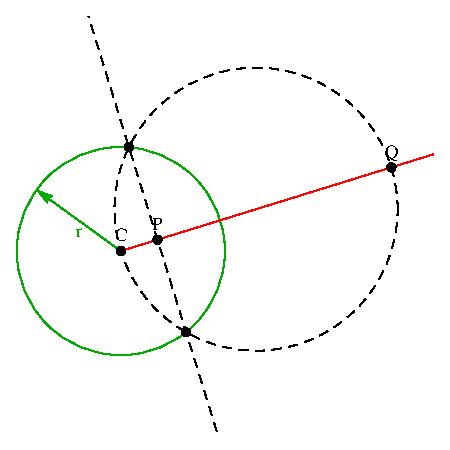
\includegraphics[width=0.5\textwidth]{figures/circ-inv}
\caption[Circle inversion]{Circle inversion with respect to the green reference circle. For a point $P$ within the reference circle the inverse $Q$ is constructed by first drawing a ray from $C$ through $P$ (red). The line normal to this ray through the point $P$ intersects the reference circle in two points. These two points together with $C$ determine a circle (dashed) which intersects the ray in the point $Q$.  The distances $CP$ and $CQ$ satisfy the relation $CP \cdot CQ = r^2$.}
\label{fig_CircInv}
\end{figure}

Coming back to the concrete map $z \mapsto \reci{z}$, it can now be interpreted the following way: Circle inversion with regard to the unit circle maps each $z \in \C$ to $\frac{z}{\abs{z}^2} = \reci{\conj{z}}$. Then reflection across the real axis (\ie complex conjugation) takes $\reci{\conj{z}}$ to $\reci{z}$. 

Summing up, all the basic types of M�bius transformations mentioned in Lemma \ref{lem_MoebiusGenerators} have a very direct geometric interpretation. Still, arbitrary M�bius transformations (especially those involving at least one inversion) are hard to describe in a similar geometric and intuitive way. Fortunately there is another characterization of M�bius transformations which is both, elegant and visually accessible.

% ---------------------------------------- Subsection: Stereographic projection
\subsection{Stereographic projection}

This section is about the great work of Douglas Arnold and Jonathan Rogness, ``M�bius transformations revealed'' \cite{arnold2008mobius}, in which the authors give a characterization of M�bius transformations in terms of stereographic projections and rigid motions of spheres 3D-space.

\todo{13}{Proof of characterization in terms of stereographic projection}


% --------------------------------------------- Subsection: Generalized circles
\subsection{Generalized circles}

\index{Generalized!circle}
From the geometric point of view M�bius transformations have the beautiful property that they preserve generalized circles. \emph{Generalized circles} are either circles (in the usual sense) or lines on the complex plane $\C$. They can also be thought of circles on the Riemann sphere (\ie the extended complex plane $\EC$ projected to the unit sphere $\UnitSphere$, see Remark~\ref{rem_RiemannSphere}), where lines on the complex plane stand in a one-to-one correspondence to circles through the point $\infty$ on the Riemann sphere. In order to give an exact definition, we follow an idea taken from \Schwerdtfeger{} and make the following considerations:

A circle with center $m \in \C$ and radius $r > 0$ can be described as the set of points $z \in \C$ for which
\begin{equation*}
\abs{z - m} = r.
\end{equation*}
This is obviously equivalent to
\begin{equation*}
\abs{z - m}^2 = (z - m) \conj{(z - m)} = r^2
\end{equation*}
and
\begin{equation}
\label{eqn_Circle}
z \conj{z} - m \conj{z} - \conj{m} z + m \conj{m} - r^2 = 0.
\end{equation}
The generalization comes into play if we multiply this last equation by a constant $A \in \R$
\begin{equation*}
A z \conj{z} - A m \conj{z} - A \conj{m} z + A m \conj{m} - A r^2 = 0
\end{equation*}
and introduce constants $B$, $C$ and $D$ appropriately such that we can write it in the form
\begin{equation}
\label{eqn_GenCircle}
A z \conj{z} + B \conj{z} + C z + D = 0.
\end{equation}
Note that $D$ is real and $B = \conj{C}$ are complex conjugates. From an equation of form (\ref{eqn_GenCircle}) we can read off the center and radius of the corresponding circle by
\begin{IEEEeqnarray}{rCl}
m &=& -\frac{B}{A}, \IEEEyessubnumber 
\label{eqn_GenCircCenter}\\
r &=& \sqrt{m \conj{m} - \frac{D}{A}} = \sqrt{\frac{BC - AD}{A^2}}. \IEEEyessubnumber 
\label{eqn_GenCircRadius}
\end{IEEEeqnarray}
Clearly we can only do so, if $A \ne 0$ and $BC - AD > 0$. 

In the case when $A = 0$, equation (\ref{eqn_GenCircle}) can be written as
\begin{equation*}
\Re{\frac{C}{\abs{C}} z} = -\frac{D}{2 \abs{C}},
\end{equation*}
which defines a line on the complex plane. We see this by considering the simpler equation $\Re{z} = -\frac{D}{2 \abs{C}}$ first (we omit the factor $\frac{C}{\abs{C}}$), which obviously defines a line parallel to the imaginary axis through the real point $-\frac{D}{2 \abs{C}}$. Then we observe that the multiplication with $\frac{C}{\abs{C}}$ just rotates this line around the origin by an angle which is given by $-\arg(C)$. 

Note that equation (\ref{eqn_GenCircle}) can also be written in matrix form:
\begin{equation*}
\rvec{\conj{z}}{1} \cdot \mat{A}{B}{C}{D} \cdot \cvec{z}{1} = 0.
\end{equation*}
If we substitute $z = u / v$, with $u,v \in \C$, $v \ne 0$ and scale by $\conj{v} \cdot v = \abs{v}^2 > 0$, we obtain the equivalent equation
\begin{equation}
\label{eqn_GenCircleMatForm}
\rvec{\conj{u}}{\conj{v}} \cdot \mat{A}{B}{C}{D} \cdot \cvec{u}{v} = 0.
\end{equation}
By introducing the convention to identify $\infty \in \EC$ with the formal quotient $u/0$, for arbitrary $u \in \C \setminus \{0\}$, equation (\ref{eqn_GenCircleMatForm}) makes sense for all $z = u/v \in \EC$. 

Finally we emphasize that the matrix in equation (\ref{eqn_GenCircleMatForm}) has a negative determinant, because of the condition $BC - AD > 0$ from above. Moreover it is a Hermitian matrix -- a notion which we will shortly recall:
\begin{definition}[Hermitian matrix]
\label{dfn_HermitianMatrix}
\index{Hermitian!matrix}
\index{Hermitian!transpose}
\index{Conjugate transpose}
Let $n > 0$ and $M \in \Mat{\C}{n}{n}$. The matrix
\begin{equation*}
\htransp{M} := \transp{\overline{M}}
\end{equation*}
obtained by complex conjugation and transposition of $M$ is called \emph{Hermitian transpose} or \emph{conjugate transpose} of $M$. If $M$ has the property $\htransp{M} = M$, it is called a \emph{Hermitian matrix}.
\end{definition}
Having now the right vocabulary and properties at hand, we can give an exact definition for generalized circles.
\begin{definition}[Generalized circle]
\index{G-circle}
\label{dfn_GenCircle}
Let $M \in \Mat{\C}{2}{2}$ be a Hermitian matrix with $\det(M) < 0$. A \emph{generalized circle}, for short \emph{g-circle}, is the set of solutions $u/v \in \EC$ with $u,v \in \C$, not both zero, to
\begin{equation}
\label{eqn_GenCircleDfn}
\rvec{\conj{u}}{\conj{v}} \cdot M \cdot \cvec{u}{v} = 0.
\end{equation}
\end{definition}

Since there should be no danger of confusion, we will from now on use the same name for a generalized circle and its corresponding Hermitian matrix (which is uniquely determined up to a nonzero real scalar factor).

\begin{remark}
Definition~\ref{dfn_GenCircle} does not depend on the choice of $u$ and $v$. If $u/v$ is a solution to (\ref{eqn_GenCircleDfn}) and $u^\prime/v^\prime = u/v$, \ie $u^\prime = \lambda u$ and $v^\prime = \lambda v$ for some $\lambda \in \C \setminus \{0\}$, then also
\begin{equation*}
\rvec{\conj{u^\prime}}{\conj{v^\prime}} \cdot M \cdot \cvec{u^\prime}{v^\prime} = \abs{\lambda}^2 \rvec{\conj{u}}{\conj{v}} \cdot M \cdot \cvec{u}{v} = 0.
\end{equation*}

Moreover we see that the point $\infty = 1/0$ lies on the g-circle $M = \smallmat{A}{B}{C}{D}$ exactly when its left upper matrix entry $A$ is zero. This is consistent with stereographic projection: The matrix entry $A$ is zero if and only if $M$ corresponds to a line on the complex plane. The image of this line under reverse stereographic projection is a circle on the Riemann sphere going through its north-pole, which we have identified with the point $\infty$.
\end{remark}

Going back to the our starting point, the equation $\abs{z - m} = r$, we can replace the equality sign `$=$' with `$<$' or `$\le$' and repeat the above considerations without any additional changes. This naturally leads to the notions of open and closed generalized disks.

\begin{definition}[Generalized disk]
\index{Generalized!disk}
\index{G-disk}
\label{dfn_GenDisk}
Let $M \in \Mat{\C}{2}{2}$ be a Hermitian matrix with $\det(M) < 0$. An \emph{open generalized disk} is the set of solutions $u/v \in \EC$, with $u,v \in \C$ -- not both zero, to
\begin{equation}
\label{eqn_GenOpenDiskDfn}
\rvec{\conj{u}}{\conj{v}} \cdot M \cdot \cvec{u}{v} < 0
\end{equation}
and a \emph{closed generalized disk} is the set of solutions $u/v \in \EC$ to
\begin{equation}
\label{eqn_GenClosedDiskDfn}
\rvec{\conj{u}}{\conj{v}} \cdot M \cdot \cvec{u}{v} \le 0.
\end{equation}
In both cases we will use the term (open/closed) \emph{g-disk} for shortness.
\end{definition}

\begin{remark}
In contrast to generalized circles, the defining matrix $M = \smallmat{A}{B}{C}{D}$ of a generalized disk is unique up to a \emph{positive} real scalar factor. Switching from $M$ to $-M$ turns the g-disk inside out while its border (the g-circle $M$) is left intact. Dependent on the sign of the left upper matrix entry $A$, we can distinguish three types of g-disks:
\begin{description}
\item[Case $A > 0$:] The g-disk corresponds to a disk in the usual sense within $\C$. Its center is given by (\ref{eqn_GenCircCenter}) and its radius by (\ref{eqn_GenCircRadius}).
\item[Case $A = 0$:] The g-disk corresponds to a half-plane of $\C$, which is obtained from the left half-plane, \ie $\Re{z} < 0$ (\resp $\le 0$), by translation by $\frac{-D}{2 \abs{C}}$ and rotation by $-\arg(C)$. The point $\infty$ is member of the generalized disk, if and only if it is closed.
\item[Case $A < 0$:] The open g-disk $M$ corresponds to the set complement (within $\EC$) of the closed g-disk $-M$ (discussed in the first case, $A > 0$). Accordingly, the closed g-disk $M$ is the complement of the open g-disk $-M$. Open and closed g-disks with $A < 0$ contain the point  $\infty$.
\end{description}
\end{remark}

It is now easy to show that g-circles and g-disks are preserved under M�bius transformations.

\begin{theorem}
\label{thm_MoebiusGenCircle}
Let $\phi$ be a M�bius transformation and $M \in \Mat{\C}{2}{2}$ be a Hermitian matrix with $\det(M) < 0$. The image of the g-circle (\resp open/closed g-disk) $M$ under the M�bius transformation $\phi$ corresponding to the matrix $P \in \GL{\C}$ is the g-circle (\resp open/closed g-disk)
\begin{equation}
\label{eqn_GDiskTransform}
\htransp{(\inv{P})} \cdot M \cdot \inv{P}.
\end{equation}
\end{theorem}
\begin{proof}
Let us write $P = \smallmat{a}{b}{c}{d}$, such that the corresponding M�bius transformation $\phi$ has the form
\begin{equation*}
\phi\left(\frac{u}{v}\right) = \frac{a u + b v}{c u + d v}.
\end{equation*}
Define $u^\prime := a u + b v$ and $v^\prime := c u + d v$. We need to show that
\begin{equation*}
\rvec{\conj{u}}{\conj{v}} \cdot M \cdot \cvec{u}{v} 
\ \left\{\ \begin{matrix} = 0 \\ < 0\\ \le 0 \end{matrix}\right.
\end{equation*}
if and only if
\begin{equation*}
\rvec{\conj{u^\prime}}{\conj{v^\prime}} \cdot \htransp{(\inv{P})} \cdot M \cdot \inv{P} \cdot \cvec{u^\prime}{v^\prime} 
\ \left\{\ \begin{matrix} = 0\phantom{.} \\ < 0\phantom{.}\\ \le 0. \end{matrix}\right.
\end{equation*}
But this follows immediately from
\begin{equation*}
P \cdot \cvec{u}{v} = \cvec{a u + b v}{c u + d v} = \cvec{u^\prime}{v^\prime}.\qedhere
\end{equation*}
\end{proof}


